\documentclass[11pt, a4paper, spanish]{article}

\usepackage[a4paper, margin=2.5cm, top=3.5cm, bottom=3.5cm]{geometry} % Define los márgenes
\usepackage{amsmath, amscd, amssymb, amsthm, latexsym, gensymb} % Paquetes matemáticos
\usepackage[spanish]{babel} % Traduce los paquetes a español
\usepackage[utf8]{inputenc} % Codificación UTF8
\usepackage{fancyhdr} % Encabezados y pies de página
  \pagestyle{fancyplain}
\usepackage{enumerate}
\usepackage{xspace}
\usepackage[page, toc]{appendix} % Apéndices
\usepackage[nottoc]{tocbibind} % Referencias en la TDC
\usepackage{scrextend} % Para usar addmargin
\usepackage{listings} % Código
  \lstdefinestyle{customcpp}{
    belowcaptionskip=1\baselineskip,
    breaklines=true,
    xleftmargin=3em,
    language=C++,
    basicstyle=\small\ttfamily
  }
\usepackage[spanish, onelanguage]{algorithm2e}
  % \NoCaptionOfAlgo
  \LinesNumbered\RestyleAlgo{ruled}\IncMargin{1em}\DontPrintSemicolon\SetArgSty{}\SetCommentSty{textsf}\SetFuncSty{textsf}
\usepackage[pdftex]{graphicx} % Imágenes
\usepackage{caratula} % Carátula del DC

% Bibliografía
\usepackage{biblatex}
\addbibresource{referencias.bib}

% Comandos personalizados
\let\strong\textbf
\renewcommand{\appendixtocname}{Apéndices}
\renewcommand{\appendixpagename}{Apéndices}
\theoremstyle{plain}
  \newtheorem{prop}{Proposición}
  \newtheorem{lema}{Lema}
\theoremstyle{remark}
  \newtheorem{obs}{Observación}
\setlength{\parskip}{.3em}

% Encabezado
\lhead{Métodos Numéricos}
\rhead{Trabajo Práctico Nº 1 - \emph{``Con 15 $\theta$s discretizo alto horno''}}
% Pie de pagina
\renewcommand{\footrulewidth}{0.4pt}
\lfoot{Grupo XX}
\rfoot{FCEN - UBA}

\begin{document}

% Datos de carátula
\materia{Métodos Numéricos}
\titulo{Trabajo Práctico Nº 1}
\subtitulo{``Con 15 $\theta$s discretizo alto horno''}
\grupo{Grupo: XX}
\fecha{Segundo cuatrimestre de 2015}

\integrante{Frizzo, Franco}{013/14}{francofrizzo@gmail.com}
\integrante{Martínez, Manuela}{160/14}{martinez.manuela.22@gmail.com}
\integrante{Rabinowicz, Lucía}{105/14}{lu.rabinowicz@gmail.com}

% Carátula
\maketitle
\newpage

% Resumen y palabras clave
\begin{addmargin}[4em]{4em}

\section*{\centering Resumen}
  El resumen, de no más de 200 palabras, deberá explicar brevemente el trabajo realizado y las conclusiones de los autores de manera que pueda ser útil por sí solo para dar una idea del contenido del trabajo.

\vspace{4em}
\noindent \strong{Palabras clave:} Las palabras clave, no más de cuatro, deben ser términos técnicos que den una idea del contenido del trabajo para facilitar su búsqueda en una base de datos temática.

\end{addmargin}
\newpage

% Índice
\tableofcontents
\newpage

% Contenido
\section{Introducción teórica}

  Contendrá una breve explicación de la base teórica que fundamenta los métodos involucrados en el trabajo, junto con los métodos mismos. No deben incluirse demostraciones de propiedades ni teoremas, ejemplos innecesarios, ni definiciones elementales (como por ejemplo la de matriz simétrica). En vez de definiciones básicas es conveniente citar ejemplos de bibliograía adecuada. \emph{Una cita vale más que mil palabras}.

  \begin{figure}[h]
    \centering
    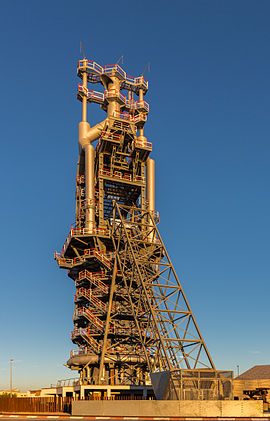
\includegraphics[width=3cm]{altoHorno.jpg}
    \caption{Podemos insertar imágenes.}
  \end{figure}

  Un alto horno es un cilindro con paredes de un cierto ancho. Dentro del mismo, se realiza la fusión de metales a temperaturas muy elevadas. Resulta útil calcular la isoterma de algún valor critico dentro de la pared, para prevenir que su estructura externa colapse.

  El objetivo del siguiente trabajo es, dadas las temperaturas internas y externas de las paredes de un alto horno y un valor, estimar la isoterma de ese valor.

  Al calcular la isoterma, se va a considerar un corte transversal de dicho horno. Para trabajar este problema computacionalmente, se discretizará el dominio en coordenadas polares.

  Se utilizará la ecuación de Laplace que permite relacionar cada punto del dominio con sus 4 vecinos. Esto genera un sistema de ecuaciones lineales que será resuelto utilizando los métodos numéricos de eliminación gaussiana y factorización LU.

  La eliminación gaussiana consiste en convertir la matriz del sistema en una matriz triangular superior y de esta forma simplificar el cálculo de las incógnitas utilizando sustitución hacia atrás.

  La factorización LU es un método similar al anterior pero no modifica el vector resultado y guarda los cambios que se le realizan a la matriz generada por el sistema al triangularla. Esto hace que para un mismo sistema de ecuaciones lineales con distintos resultados no sea necesario recalcular para cada uno la matriz triangulada, si  no que se realiza solo una vez y luego se afecta al vector resultado con los cambios guardados.

  % Ecuación de Laplace
  % Buscar citas en libros sobre eliminación gaussiana y factorización LU

\section{Desarrollo}

  Deben explicarse los métodos numéricos que utilizaron y su aplicación al problema concreto involucrado en el trabajo práctico. Se deben mencionar los pasos que siguieron para implementar los algoritmos, las dificultades que fueron encontrando y la descripción de cómo las fueron resolviendo. Explicar también cómo fueron planteadas y realizadas las mediciones experimentales.\footnote{Podemos hacer notas al pie.} Los ensayos fallidos, hipótesis y conjeturas equivocadas, experimentos y métodos malogrados deben figurar en esta sección, con una breve explicación de los motivos de estas fallas (en caso de ser conocidas).

  Dados los parámetros de entrada, creamos una matriz asociada al sistema relacionando cada uno de los puntos del dominio con sus vecinos a través de la ecuación de Laplace.

  % Así formamos una matriz diagonal dominante, lo que nos permite asegurarnos que el método de eliminación gaussiana se va a poder llevar a cabo sin necesidad de intercambiar filas, es decir, sin pivoteo.

  \subsection{Planteo del sistema y métodos numéricos aplicados}

    \subsubsection*{Demostración de que puede aplicarse Eliminación Gaussiana en el sistema estudiado}

      Para poder utilizar los métodos elegidos para resolver el problema, necesitamos asegurarnos de que estos son aplicables en este caso en particular. Bastará con asegurarnos de poder aplicar Eliminación Gaussiana sin pivoteo, ya que esto implica que también podremos calcular la factorización LU de la matriz del sistema.\cite[p.~403]{burden}

      En primer lugar, notemos que la matriz $A \in \mathbb{R}^{(m+1)n \times (m+1)n}$ es diagonal dominante, de manera no estricta. En efecto:

      \begin{itemize}

        \item Para las filas $1$ a $n$ de la matriz, correspondientes al borde interno de la discretización, y $mn + 1 $ a $(m+1)n$, correspondientes al borde externo, tenemos que
          \[ A_{p,q} = \begin{cases}
            1 & \text{si $p = q$} \\
            0 & \text{si $p \neq q$}
          \end{cases} \]
        Por lo tanto,
          \[ \vert A_{p,p} \vert = 1 \geq 0 = \sum_{\substack{q=1 \\ q \neq p}}^{(m+1)n} \vert A_{p,q} \vert \]

        \item Las filas $n + 1$ a $mn$ de la matriz corresponden a los puntos $t_{j,k}$ de la discretización con $1 \leq j < m$. En todos estos casos, encontramos solo 5 coeficientes no nulos en la $p$-ésima fila, siendo el que aparece en la diagonal el correspondiente a la variable $t_{j,k}$, y por lo tanto
          \[ \begin{split}
            \vert A_{p,p} \vert &= \left \vert - \frac{2}{(\Delta r)^2} + \frac{1}{r \Delta r} - \frac{2}{r^2 (\Delta \theta)^2} \right \vert \\
            &= \left \vert - \frac{1}{(\Delta r)^2} + \frac{1}{r \Delta r} - \frac{2}{r^2 (\Delta \theta)^2} - \frac{1}{(\Delta r)^2} \right \vert \\
            &= \left \vert - \frac{r - \Delta r}{r (\Delta r)^2} - \frac{2}{r^2 (\Delta \theta)^2} - \frac{1}{(\Delta r)^2} \right \vert \\
            &= \left \vert \frac{r - \Delta r}{r (\Delta r)^2} + \frac{2}{r^2 (\Delta \theta)^2} + \frac{1}{(\Delta r)^2} \right \vert
          \end{split} \]

        Teniendo en cuenta que
          \[ r - \Delta r = (r_i + j \Delta r) - \Delta r = r_i + (j - 1) \Delta r > 0\]
        dado que $r_i, \Delta r > 0$ y $j \geq 1$, es fácil notar que todos los términos que aparecen dentro del módulo son positivos, y por lo tanto
          \[ \vert A_{p,p} \vert = \frac{r - \Delta r}{r (\Delta r)^2} + \frac{2}{r^2 (\Delta \theta)^2} + \frac{1}{(\Delta r)^2} \]

        Por otro lado
          \[ \begin{split}
            \sum_{\substack{q=1 \\ q \neq p}}^{(m+1)n} \vert A_{p,q} \vert &= \left \vert \frac{1}{(\Delta r)^2} - \frac{1}{r \Delta r} \right \vert + 2 \left \vert \frac{1}{r^2 (\Delta \theta)^2} \right \vert + \left \vert \frac{1}{(\Delta r)^2} \right \vert \\
            &= \left \vert \frac{r - \Delta r}{r (\Delta r)^2} \right \vert + \frac{2}{r^2 (\Delta \theta)^2} + \frac{1}{(\Delta r)^2} \\
            &= \frac{r - \Delta r}{r (\Delta r)^2} + \frac{2}{r^2 (\Delta \theta)^2} + \frac{1}{(\Delta r)^2} = \vert A_{p,p} \vert
          \end{split} \]

      \end{itemize}

      De lo anterior, se sigue que
        \[ \vert A_{p,p} \vert \geq \sum_{\substack{q=1 \\ q \neq p}}^{(m+1)n} \vert A_{p,q} \vert \qquad \text{para todo $p = 1, \dots, (m+1)n$} \]
      es decir, $A$ es diagonal dominante de forma no estricta.

      \begin{obs}
        \label{obs:Diagonal de A sin ceros}
        Para todo $p = 1, \dots, (m+1)n$, $\vert A_{p,p} \vert > 0$, i.e. la diagonal de $A$ no contiene ceros.
      \end{obs}

      A continuación, probaremos un resultado que nos será útil: al realizar el primer paso de Eliminación Gaussiana sobre una matriz diagonal dominante, la matriz resultante también lo es.

      \begin{lema}
        \label{lema:EG conserva diagonal dominante}
        Sea $A^{(0)} = A \in \mathbb{R}^{n \times n}$ una matriz diagonal dominante, y $A^{(1)}$ el resultado de aplicar un paso de Eliminación Gaussiana (sin pivoteo) sobre $A$. Entonces $A^{(1)}$ es diagonal dominante.
      \end{lema}
      \begin{proof}
        Consideremos la fila $i$-ésima de $A^{(1)}$, y veamos que $\left \vert A^{(1)}_{i,i} \right \vert \geq \sum_{\substack{j = 1 \\ j \neq i}}^n \left \vert A^{(1)}_{i,j} \right \vert$. Tenemos que
        \[ \left \vert A^{(1)}_{i,i} \right \vert = \left \vert A_{i,i} - \frac{A_{i,1}}{A_{1,1}} A_{1,i} \right \vert
          \qquad \text{y} \qquad
        \sum_{\substack{j = 1 \\ j \neq i}}^n \left \vert A^{(1)}_{i,j} \right \vert
          = \sum_{\substack{j = 2 \\ j \neq i}}^n \left \vert A_{i,j} - \frac{A_{i,1}}{A_{1,1}} A_{1,j} \right \vert \]

        Luego,

        \[ \begin{split}
          \sum_{\substack{j = 1 \\ j \neq i}}^n \left \vert A^{(1)}_{i,j} \right \vert
          &= \sum_{\substack{j = 2 \\ j \neq i}}^n \left \vert A_{i,j} - \frac{A_{i,1}}{A_{1,1}} A_{1,j} \right \vert \\
          &\leq \sum_{\substack{j = 2 \\ j \neq i}}^n \vert A_{i,j} \vert + \left \vert \frac{A_{i,1}}{A_{1,1}} \right \vert \sum_{\substack{j = 2 \\ j \neq i}}^n \vert A_{1,j} \vert \\
          &\leq \left( \vert A_{i,i} \vert - \vert A_{i,1} \vert \right) + \left \vert \frac{A_{i,1}}{A_{1,1}} \right \vert \left( \vert A_{1,1} \vert - \vert A_{1,i} \vert \right) \\
          &= \vert A_{i,i} \vert - \left \vert \frac{A_{i,1}}{A_{1,1}} \right \vert \vert A_{1,i} \vert \\
          &\leq \left \vert A_{i,i} -  \frac{A_{i,1}}{A_{1,1}} A_{1,i} \right \vert = \left \vert A^{(1)}_{i,i} \right \vert
        \end{split} \]
      \end{proof}

      Consideremos de nuevo la matriz $A \in \mathbb{R}^{(m+1)n \times (m+1)n}$ correspondiente al sistema estudiado. Probemos ahora que es posible aplicar Eliminación Gaussiana sin pivoteo. Más especificamente, probaremos que para $u \leq (m+1)n$, es posible realizar $u$ iteraciones de Eliminación Gaussiana sobre $A$ sin pivoteo, y que luego de las mismas, la matriz $A^{(u)}$ resultante es diagonal dominante, con su fila $u + 1$ no nula.

      \begin{proof}
        Lo haremos por inducción en $u$. 
        \begin{itemize}
          \item[\textbf{C.B.}] Teniendo en cuenta que la primera fila de la matriz $A$ tiene necesariamente un $1$ en la diagonal y $0$ en las demás posiciones, se deduce trivialmente que es posible aplicar el primer paso de Eliminación Gaussiana sin realizar pivoteo, dado que $A_{1, 1}$ es no nulo. Del Lema \ref{lema:EG conserva diagonal dominante}, se sigue que la matriz $A^{(1)}$ obtenida será diagonal dominante. Como $A_{1, 2} = 0$, tendremos $A^{(1)}_{2,2} = A_{2,2}$, que es necesariamente no nulo (Observación \ref{obs:Diagonal de A sin ceros}), por lo que la segunda fila de $A^{(1)}$ será no nula.
              
          \item[\textbf{P.I.}] Supongamos que la matriz $A^{(u - 1)}$, obtenida tras aplicar $u - 1$ pasos de Eliminación Gaussiana sobre $A$, es diagonal dominante, con su $u$-ésima fila no nula. Esto implica que $A^{(u - 1)}_{u,u} \neq 0$. Notemos que podemos escribir a $A^{(u - 1)}$ por bloques de la siguiente manera
            \[ A^{(u - 1)} = \left( \begin{matrix} U_{u - 1} & B \\ 0 & \widetilde{A}_{u - 1} \end{matrix} \right) \]
          donde las matrices $U_{u - 1} \in \mathbb{R}^{(u-1)\times(u-1)}$ y $\widetilde{A}_{u - 1} \in \mathbb{R}^{(n-u+1)\times(n-u+1)}$ son trivialmente diagonal dominantes.

          Podemos ver que realizar el paso $u$-ésimo del algoritmo de Eliminación Gaussiana sobre $A$ equivale a realizar el primer paso de este algoritmo sobre $\widetilde{A}_{u - 1}$, sin modificar el resto de la matriz. Dado que $A^{(u - 1)}_{u,u} \neq 0$, podremos realizar esto sin pivoteo, y del Lema 1 se sigue que el resultado de este proceso será diagonal dominante, lo cual implica directamente que también lo será $A^{(u)}$.

          Por último, probemos que la fila $u + 1$ de la matriz $A^{(u)}$ es no nula.
          \begin{itemize}
            \item Si $1 \leq u + 1 \leq n$ o $mn < u + 1 \leq (m+1)n$, tendremos que la fila $u + 1$ tendrá un $1$ en la diagonal y $0$ en las demás posiciones, por lo que no se verá afectada por el algoritmo de Eliminación Gaussiana. Luego $A^{(u)}_{u+1,u+1} = 1$.
            \item En caso contrario, por la forma en la que se construye la matriz del sistema, $A_{u+1,u+1+n}$ corresponde al coeficiente de la variable $t_{j,k+1}$ de la $u + 1$-ésima ecuación del sistema, que es trivialmente no nulo. Además, la matriz $A$ es banda $n, n$, como se demuestra en el Anexo C. Por lo tanto, $A_{p,u+1+n} = 0$ para todo $p = 0, \dots, u$ y, por consiguiente, $A^{(u)}_{u+1,u+1+n} = A_{u+1,u+1+n}$. Esto implica que la fila $u + 1$ de la matriz $A^{(u)}$ es no nula, como queríamos probar. \qedhere
          \end{itemize}
        \end{itemize}
      \end{proof}

  \subsection{Implementación de los métodos}

  \subsection{Estimación de la posición de la isoterma y medida de la peligrosidad}

    Una vez obtenida la resolución del sistema, fue necesario decidir un criterio para estimar la ubicación de la isoterma pedida. Algunas de las alternativas que consideramos al respecto fueron las siguientes:

    \begin{itemize}
      \item Para cada ángulo $\theta_k$, considerar como posición de la isoterma el radio correspondiente al punto $(r_j, \theta_k)$ de la discretización con el valor de $t_{j,k}$ más próximo a 500{\degree}C.
      \item Para cada ángulo $\theta_k$, considerar como posición de la isoterma el radio del punto de la discretización inmediatamente exterior al primero con temperatura mayor o igual a 500{\degree}C, contando desde la pared externa. Es decir, considerar el menor radio $r_j$ tal que $t_{j',k} < 500$ para todo $j' \geq j$. La ventaja de este método es que asegura que la isoterma nunca se encontrará más cerca de la pared externa que el resultado arrojado, garantizando que se detectarán todas las posibles situaciones de riesgo.
      \item Para cada ángulo $\theta_k$, considerar $r_j$, el radio del punto más externo de la discretización con temperatura mayor o igual a 500{\degree}C. Luego, sabiendo que la isoterma buscada se encontrará entre este radio y el inmediatamente exterior, aproximar la variación de la temperatura en los puntos intermedios mediante una función lineal y utilizar esta aproximación para estimar la posición de la isoterma. Más precisamente, si $r_{iso}$ es el radio de la isoterma buscada, entonces
        \[ r_{iso} = r_j + \Delta r \left(\frac{500 - t_{j,k}}{t_{j+1,k} - t_{j,k}} \right) \]
    \end{itemize}

    Finalmente, decidimos aplicar este último criterio, porque consideramos que brinda información más precisa que los otros dos, al tener en cuenta el valor la diferencia de temperatura entre los puntos de la discretización más cercanos a la isoterma buscada y la isoterma en si misma, información que los dos primeros métodos descartan. De esta manera, nos permite detectar situaciones de riesgo que con el primer método pasarían desapercibidas, pero evitando la generación de falsos positivos que provocaría el segundo método, que es mucho más estricto.

  \subsection{Hipótesis planteadas}

    Suponemos que lo que va a pasar es que cuanto mas instancias haya en el sistema, mas diferencia va a haber entre los métodos numéricos a utilizar. El método de eliminación gaussiana es mas lento cuando aumentan las instancias ya que para cada una de ellas recalcula todo el sistema. En cambio, el método de factorización LU calcula la factorización LU del sistema una única vez y después modifica en base a este los parámetros de entrada para calcular el sistema total. Mientras que cuando hay pocas instancias el tiempo que tomarán va a ser muy similar. Eliminación gaussiana para una única instancia es un poco mas rápido que LU ya que no podemos sacar la ventaja de guardar la factorización LU para no recalcular la matriz del sistema cuando es un único sistema y a pesar de tener un orden similar, factorización LU supera a eliminación gaussiana por una constante.

  \subsection{Mediciones experimentales realizadas}


\section{Resultados}

  Deben incluir los resultados de los experimentos, utilizando el formato más adecuado para su presentación. Deberán especificar claramente a qué experiencia corresponde cada resultado. No se incluirán aquí corridas de máquina.

\section{Discusión}

  Se incluirá aquí un análisis de los resultados obtenidos en la sección anterior (se analizará su validez, coherencia, etc.). Deben analizarse como mínimo los ítems pedidos en el enunciado. No es aceptable decir que ``los resultados fueron los esperados'', sin hacer clara referencia a la teoría a la cual se ajustan. Además, se deben mencionar los resultados interesantes y los casos ``patológicos'' encontrados.

\section{Conclusiones}

  Esta sección debe contener las conclusiones generales del trabajo. Se deben mencionar las relaciones de la discusión sobre las que se tiene certeza, junto con comentarios y observaciones generales aplicables a todo el proceso. Mencionar también posibles extensiones a los métodos, experimentos que hayan quedado pendientes, etc.

  \begin{enumerate}
    \item Podemos hacer listas numeradas
    \item ¡Con más de un item!
  \end{enumerate}

  \begin{itemize}
    \item Incluso podemos hacer
    \item listas con viñetas
    \item :D
  \end{itemize}

\newpage
\begin{appendices}

  \section{Enunciado del trabajo práctico}

    \subsection{Introducción}

      Consideremos la sección horizontal de un horno de acero cilíndrico, como en la Figura \ref{fig:seccionHorno}. El sector A es la pared del horno, y el sector B es el horno propiamente dicho, en el cual se funde el acero a temperaturas elevadas. Tanto el borde externo como el borde interno de la pared forman círculos. Suponemos que la temperatura del acero dentro del horno (o sea, dentro de B) es constante e igual a 1500{\degree}C.
      Tenemos sensores ubicados en la parte externa del horno para medir la temperatura de la pared externa del mismo, que habitualmente se encuentra entre 50{\degree}C y 200{\degree}C. El problema que debemos resolver consiste en estimar la isoterma de 500{\degree}C dentro de la pared del horno, para estimar la resistencia de la misma. Si esta isoterma está demasiado cerca de la pared externa del horno, existe peligro de que la estructura externa de la pared colapse.

      \begin{figure}[h]
        \centering
        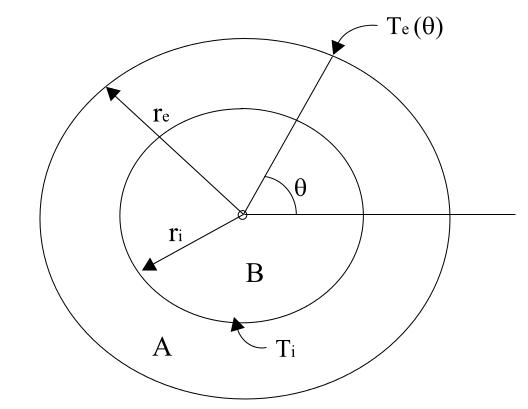
\includegraphics[width=10cm]{seccionHorno.jpg}
        \caption{Sección circular del horno.}
        \label{fig:seccionHorno}
      \end{figure}

      El objetivo del trabajo práctico es implementar un programa que calcule la isoterma solicitada, conociendo las dimensiones del horno y las mediciones de temperatura en la pared exterior.

    \subsection{El Modelo}

      Sea $r_e \in \mathbb{R}$ el radio exterior de la pared y sea $r_i \in \mathbb{R}$ el radio interior de la pared. Llamemos $T(r, \theta)$ a la temperatura en el punto dado por las coordenadas polares $(r, \theta)$, siendo $r$ el radio y $\theta$ el ángulo polar de dicho punto. En el estado estacionario, esta temperatura satisface la ecuación del calor:

      \begin{equation} \label{eq:en1}
        \frac{\partial^2 T(r, \theta)}{\partial r^2} + \frac{1}{r} \frac{\partial T(r, \theta)}{\partial r} + \frac{1}{r^2} \frac{\partial^2 T(r, \theta)}{\partial \theta^2} = 0
      \end{equation}

      Si llamamos $T_i \in \mathbb{R}$ a la temperatura en el interior del horno (sector B) y $T_e : [0, 2\pi] \to \mathbb{R}$ a la función de temperatura en el borde exterior del horno (de modo tal que el punto $(r_e, \theta)$ tiene temperatura $T_e(\theta)$), entonces tenemos que

      \begin{equation} \label{eq:en2}
        T(r, \theta) = T_i \text{ para todo punto } (r, \theta) \text{ con } r \leq r_i
      \end{equation}

      \begin{equation} \label{eq:en3}
        T(r_e, \theta) = T_e(\theta) \text{ para todo punto } (r_e, \theta)
      \end{equation}

      El problema en derivadas parciales dado por la primera ecuación con las condiciones de contorno presentadas recientemente, permite encontrar la función $T$ de temperatura en el interior del horno (sector A), en función de los datos mencionados en esta sección.

      Para resolver este problema computacionalmente, discretizamos el dominio del problema (el sector A) en coordenadas polares. Consideramos una partición $0 = \theta_0 < \theta_1 < ... < \theta_n = 2\pi$ en $n$ ángulos discretos con $\theta_k - \theta_{k-1} = \Delta \theta$ para $k = 1, \dots n$, y una partición $r_i = r_0 < r_1 < ... < r_m = r_e$ en $m + 1$ radios discretos con $r_j - r_{j-1} = \Delta r$ para $j = 1, \dots m$.

      El problema ahora consiste en determinar el valor de la función $T$ en los puntos de la discretización $(r_j, \theta_k)$ que se encuentren dentro del sector A. Llamemos $t_{jk} = T(r_j , \theta_k)$ al valor (desconocido) de la función $T$ en el punto $(r_j, \theta_k)$.

      Para encontrar estos valores, transformamos la ecuación (\ref{eq:en1}) en un conjunto de ecuaciones lineales sobre las incógnitas $t_{jk}$, evaluando (\ref{eq:en1}) en todos los puntos de la discretización que se encuentren dentro del sector A. Al hacer esta evaluación, aproximamos las derivadas parciales de $T$ en (\ref{eq:en1}) por medio de las siguientes fórmulas de diferencias finitas:

      \begin{equation} \label{eq:en4}
        \frac{\partial^2 T(r, \theta)}{\partial r^2}(r_j, \theta_k) \cong \frac{t_{j-1,k} - 2 t_{jk} + t_{j+1,k}}{(\Delta r)^2}
      \end{equation}

      \begin{equation} \label{eq:en5}
        \frac{\partial T(r, \theta)}{\partial r}(r_j, \theta_k) \cong \frac{t_{j,k} - t_{j-1,k}}{\Delta r}
      \end{equation}

      \begin{equation} \label{eq:en6}
        \frac{\partial^2 T(r, \theta)}{\partial \theta^2}(r_j, \theta_k) \cong \frac{t_{j,k-1} - 2 t_{jk} + t_{j,k+1}}{(\Delta \theta)^2}
      \end{equation}

      Es importante notar que los valores de las incógnitas son conocidos para los puntos que se encuentran sobre el borde exterior de la pared, y para los puntos que se encuentren dentro del sector B. Al realizar este procedimiento, obtenemos un sistema de ecuaciones lineales que modela el problema discretizado. La resolución de este sistema permite obtener una aproximación de los valores de la función $T$ en los puntos de la discretización.

    \subsection{Enunciado}
      Se debe implementar un programa en \texttt{C} o \texttt{C++} que tome como entrada los parámetros del problema ($r_i$, $r_e$, $m + 1$, $n$, valor de la isoterma buscada, $T_i$, $T_e(\theta)$) que calcule la temperatura dentro de la pared del horno utilizando el modelo propuesto en la sección anterior y que encuentre la isoterma buscada en función del resultado obtenido del sistema de ecuaciones. El método para determinar la posición de la isoterma queda a libre elección de cada grupo y debe ser explicado en detalle en el informe.

      El programa debe formular el sistema obtenido a partir de las ecuaciones (\ref{eq:en1})-(\ref{eq:en6}) y considerar dos métodos posibles para su resolución: mediante el algoritmo clásico de Eliminación Gaussiana y la Factorización LU. Finalmente, el programa escribirá en un archivo la solución obtenida con el formato especificado en la siguiente sección.

      Como ya se ha visto en la materia, no es posible aplicar los métodos propuestos para la resolución a cualquier sistema de ecuaciones. Sin embargo, la matriz del sistema considerado en el presente trabajo cumple con ser diagonal dominante (no estricto) y que, ordenando las variables y ecuaciones convenientemente, es posible armar un sistema de ecuaciones cuya matriz posee la propiedad de ser \emph{banda}. Luego, se pide demostrar (o al menos dar un esquema de la demostración) el siguiente resultado e incluirlo en el informe:

      \begin{prop}
        Sea $A \in \mathbb{R}^{n \times n}$ la matriz obtenida para el sistema definido por (\ref{eq:en1})-(\ref{eq:en6}). Demostrar que es posible aplicar Eliminación Gaussiana sin pivoteo.\footnote{Sugerencia: Notar que la matriz es diagonal dominante (no estrictamente) y analizar qué sucede al aplicar un paso de Eliminación Gaussiana con los elementos de una fila.}
      \end{prop}

      La solución del sistema de ecuaciones permitirá saber la temperatura en los puntos de la discretización. Sin embargo, nuestro interés es calcular la isoterma 500, para poder determinar si la estructura se encuentra en peligro. Luego, se pide lo siguiente:

      \begin{itemize}
        \item Dada la solución del sistema de ecuaciones, proponer una forma de estimar en cada ángulo de la discretización la posición de la isoterma 500.
        \item En función de la aproximación de la isoterma, proponer una forma (o medida) a utilizar para evaluar la peligrosidad de la estructura en función de la distancia a la pared externa del horno.
      \end{itemize}

      En función de la experimentación, se busca realizar dos estudios complementarios: por un lado, analizar cómo se comporta el sistema y, por otro, cuáles son los requerimientos computacionales de los métodos. Se pide como mínimo realizar los siguientes experimentos:

      \begin{enumerate}
        \item Comportamiento del sistema.
          \begin{itemize}
            \item Considerar al menos dos instancias de prueba, generando distintas discretizaciones para cada una de ellas y comparando la ubicación de la isoterma buscada respecto de la pared externa del horno. Se sugiere presentar gráficos de temperatura o curvas de nivel para los mismos, ya sea utilizando las herramientas provistas por la cátedra o implementando sus propias herramientas de graficación.
            \item Estudiar la proximidad de la isoterma buscada respecto de la pared exterior del horno en función de distintas granularidades de discretización y las condiciones de borde.
          \end{itemize}

        \item Evaluación de los métodos.
          \begin{itemize}
            \item Analizar el tiempo de cómputo requerido para obtener la solución del sistema en función de la granularidad de la discretización. Se sugiere presentar los resultados mediante gráficos de tiempo de cómputo en función de alguna de las variables del problema.
            \item Considerar un escenario similar al propuesto en el experimento 1. pero donde las condiciones de borde (i.e., $T_i$ y $T_e(\theta)$) cambian en distintos instantes de tiempo. En este caso, buscamos obtener la secuencia de estados de la temperatura en la pared del horno, y la respectiva ubicación de la isoterma especificada. Para ello, se considera una secuencia de $ninst$ vectores con las condiciones de borde, y las temperaturas en cada estado es la solución del correspondiente sistema de ecuaciones. Se pide formular al menos un experimento de este tipo, aplicar los métodos de resolución propuestos de forma conveniente y compararlos en términos de tiempo total de cómputo requerido para distintos valores de $ninst$.
          \end{itemize}
      \end{enumerate}

      De manera opcional, aquellos grupos que quieran ir un poco más allá pueden considerar trabajar y desarrollar alguno(s) de los siguientes puntos extra:
      \begin{enumerate}
        \item Notar que el sistema resultante tiene estructura \emph{banda}. Proponer una estructura para aprovechar este hecho en términos de la \emph{complejidad espacial} y como se adaptarían los algoritmos de Eliminación Gaussiana y Factorización LU para reducir la cantidad de operaciones a realizar.
        \item Implementar dicha estructura y las adaptaciones necesarias para el algoritmo de Eliminación Gaussiana.
        \item Implementar dicha estructura y las adaptaciones necesarias para el algoritmo de Factorización LU.
      \end{enumerate}

      Finalmente, se deberá presentar un informe que incluya una descripción detallada de los métodos implementados y las decisiones tomadas, el método propuesto para el cálculo de la isoterma buscada y los experimentos realizados, junto con el correspondiente análisis y siguiendo las pautas definidas en el archivo \texttt{pautas.pdf}.

    \subsection{Programa y formato de archivos}
      Se deberán entregar los archivos fuentes que contengan la resolución del trabajo práctico. El ejecutable tomará tres parámetros por línea de comando, que serán el archivo de entrada, el archivo de salida, y el método a ejectutar (0 Eliminación Gaussiana, 1 LU).

      El archivo de entrada tendrá la siguiente estructura:
      \begin{itemize}
        \item La primera línea contendrá los valores $r_i$, $r_e$, $m + 1$, n, iso, $ninst$, donde $iso$ representa el valor de la isoterma buscada y $ninst$ es la cantidad de instancias del problema a resolver para los parámetros dados.
        \item A continuación, el archivo contendrá $ninst$ líneas, cada una de ellas con $2 n$ valores, los primeros $n$ indicando los valores de la temperatura en la pared interna, i.e., $T_i(\theta_0), T_i(\theta_1), \dots, T_i(\theta_n-1)$, seguidos de $n$ valores de la temperatura en la pared externa, i.e., $T_e(\theta_0), T_e(\theta_1), \dots, T_e(\theta_n-1)$.
      \end{itemize}

      El archivo de salida obligatorio tendrá el vector solución del sistema reportando una componente del mismo por línea. En caso de $ninst > 1$, los vectores serán reportados uno debajo del otro.

      Junto con el presente enunciado, se adjunta una serie de scripts hechos en \texttt{python} y un conjunto instancias de test que deberán ser utilizados para la compilación y un testeo básico de la implementación. Se recomienda leer el archivo \texttt{README.txt} con el detalle sobre su utilización.

    \subsection{Fechas de entrega}
      \begin{itemize}
        \item \emph{Formato Electrónico}: Jueves 3 de Septiembre de 2015, hasta las 23:59 hs, enviando el trabajo (informe + código) a la dirección \texttt{metnum.lab@gmail.com}. El subject del email debe comenzar con el texto \texttt{[TP1]} seguido de la lista de apellidos de los integrantes del grupo.
        \item \emph{Formato físico}: Viernes 4 de Septiembre de 2015, de 17:30 a 18:00 hs.
      \end{itemize}

      \strong{Importante}: El horario es estricto. Los correos recibidos después de la hora indicada serán considerados re-entrega. Los grupos deben ser de 3 o 4 personas, sin excepción. Es indispensable que los trabajos pasen satisfactoriamente los casos de test provistos por la cátedra.

  \newpage
  \section{Código fuente}

    En el apéndice B se incluirán los códigos fuente de las funciones relevantes desde el punto de vista numérico.

    \begin{algorithm}
      \caption{Podemos escribir pseudocódigo}
      \While{true}{
        $a \gets b$ \;
      }
    \end{algorithm}

    También podemos incluir archivos de código:
    \lstinputlisting[language=C++, firstline=0, lastline=18, style=customcpp]{../src/altohorno.cpp}

  \newpage
  \section{Otras cosillas}

    Resultados que valga la pena mencionar en el trabajo pero que sean demasiado específicos para aparecer en el cuerpo principal del trabajo podrán mencionarse en sucesivos apéndices rotulados con las letras mayusculas del alfabeto romano. Por ejemplo: la demostración de una propiedad que aplican para optimizar el algoritmo que programaron para resolver un problema.

\end{appendices}

\newpage

\printbibliography[heading=bibintoc]

  Es importante incluir referencias a libros, artículos y páginas de Internet consultados durante el desarrollo del trabajo, haciendo referencia a estos materiales a lo largo del informe.
  Se deben citar también las comunicaciones personales con otros grupos.

\end{document}
